\begin{figure}[ht!]
  \centering
  \subfigure[$p_T^V$ 2tag 2jet
  bb]{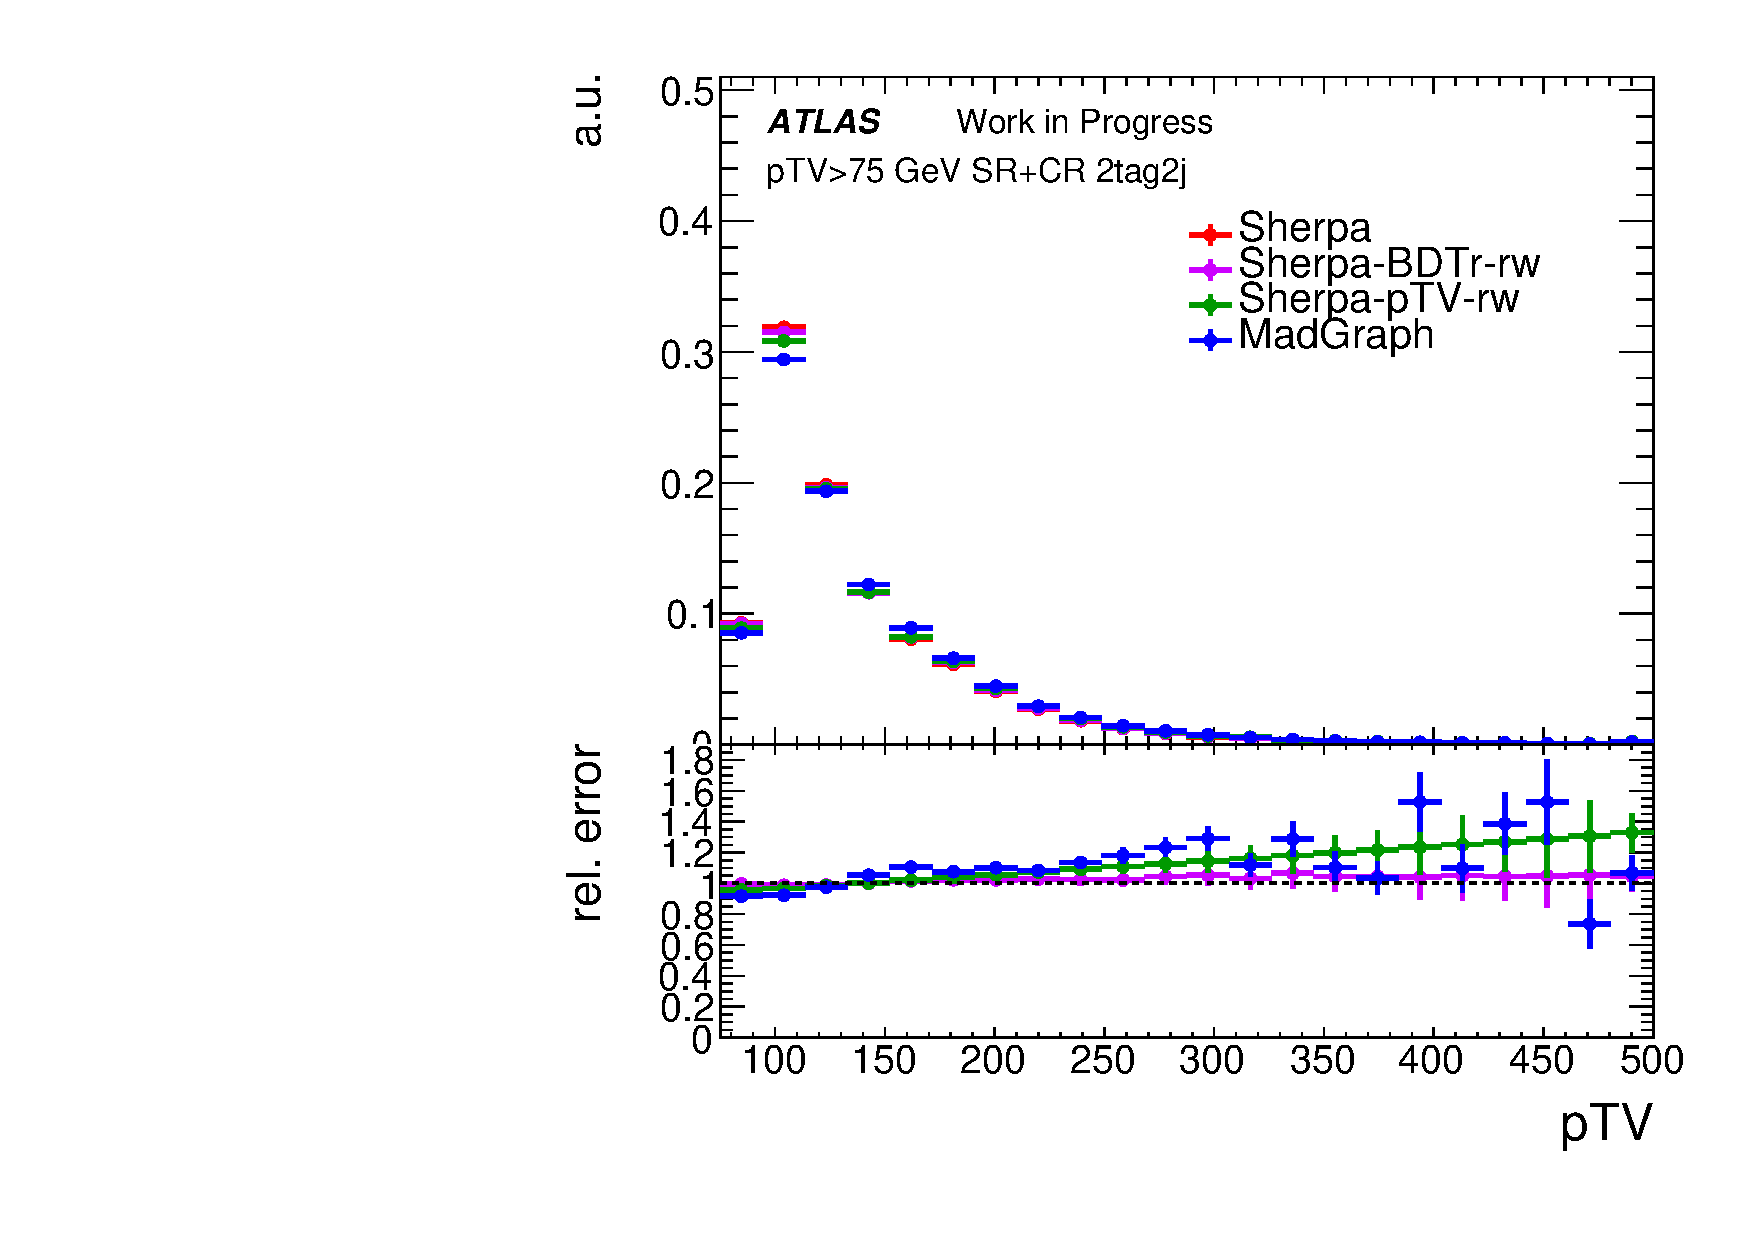
\includegraphics[width=0.45\textwidth]{1Lep_pTVreweighting_shapes/1lepton_2tag2jet_75ptv_SR+CR_pTV_bb.pdf}}
  \subfigure[$p_T^V$ 2tag 2jet
  bc]{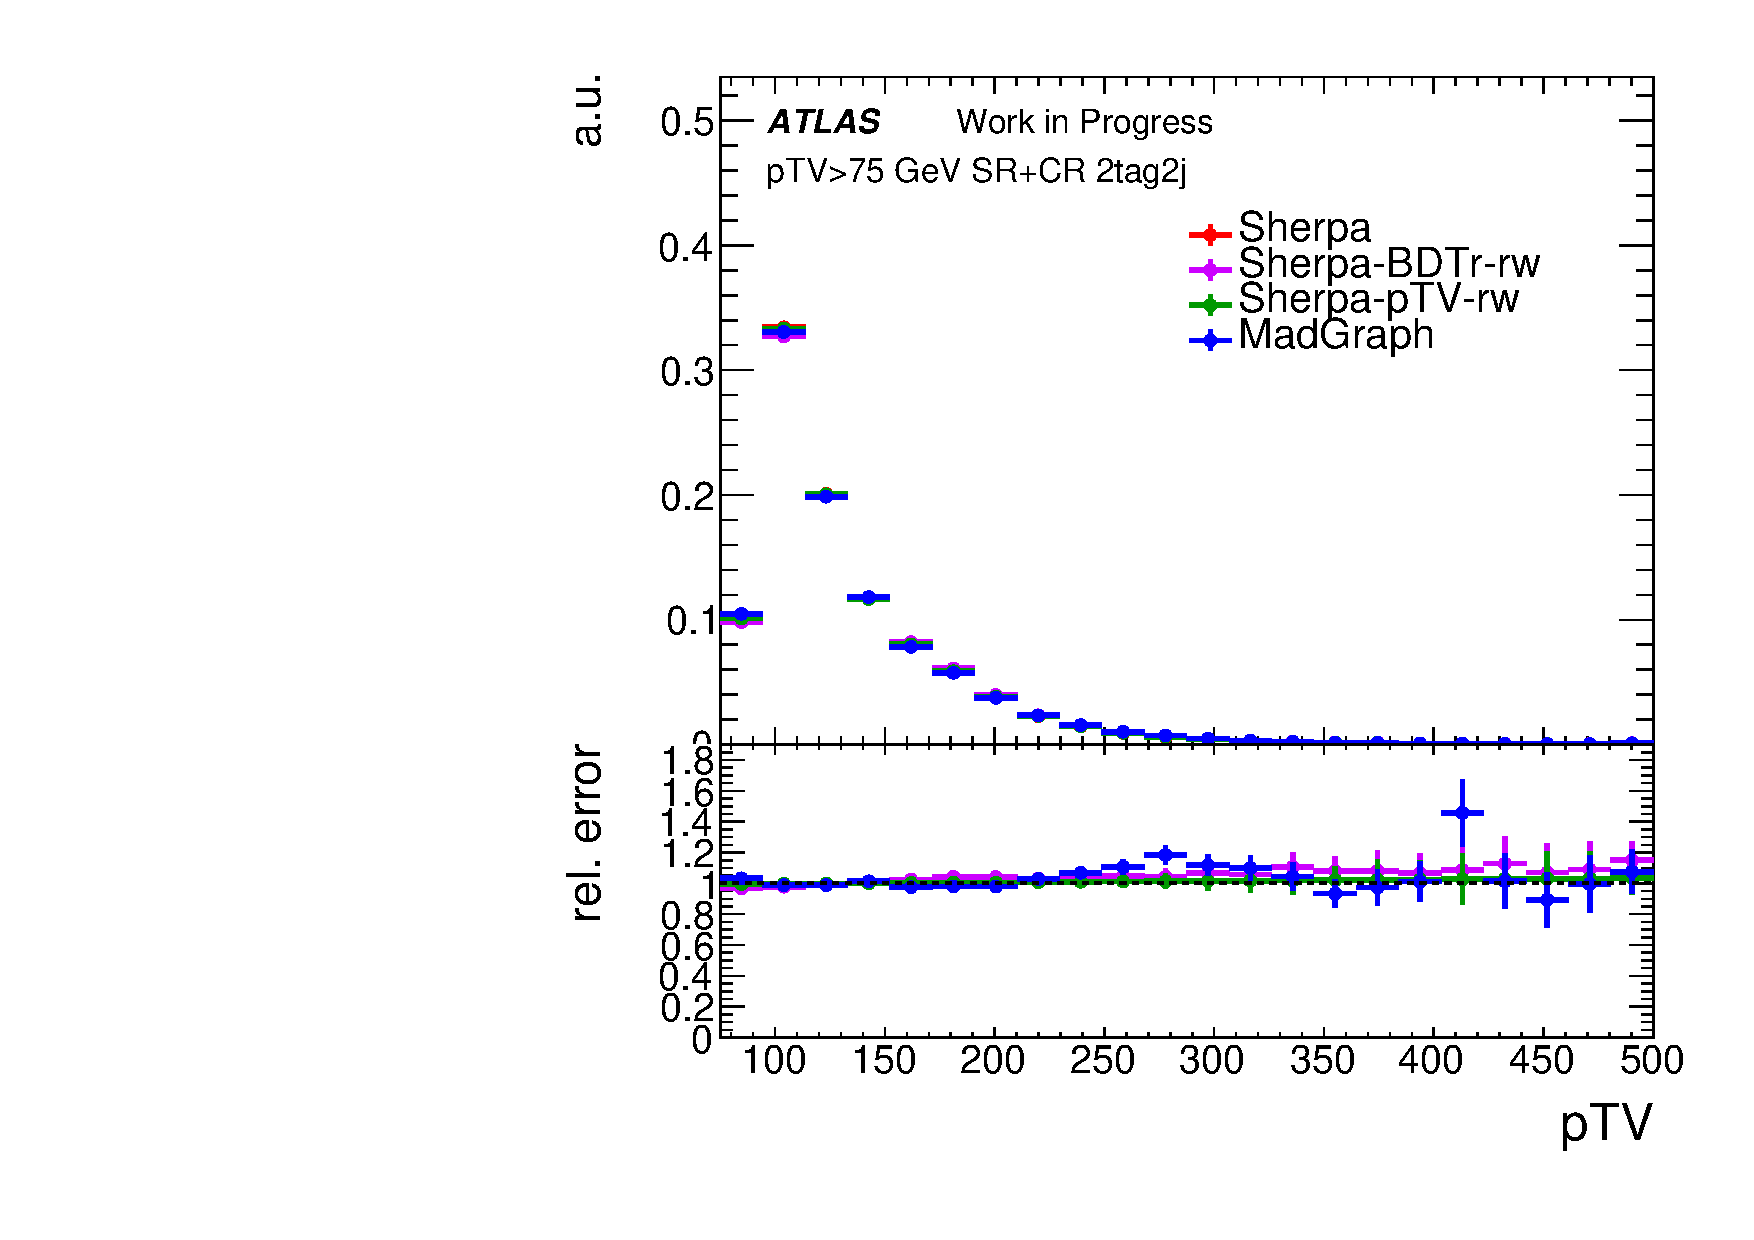
\includegraphics[width=0.45\textwidth]{1Lep_pTVreweighting_shapes/1lepton_2tag2jet_75ptv_SR+CR_pTV_bc.pdf}}
  \\
  \subfigure[$p_T^V$ 2tag 2jet bl]{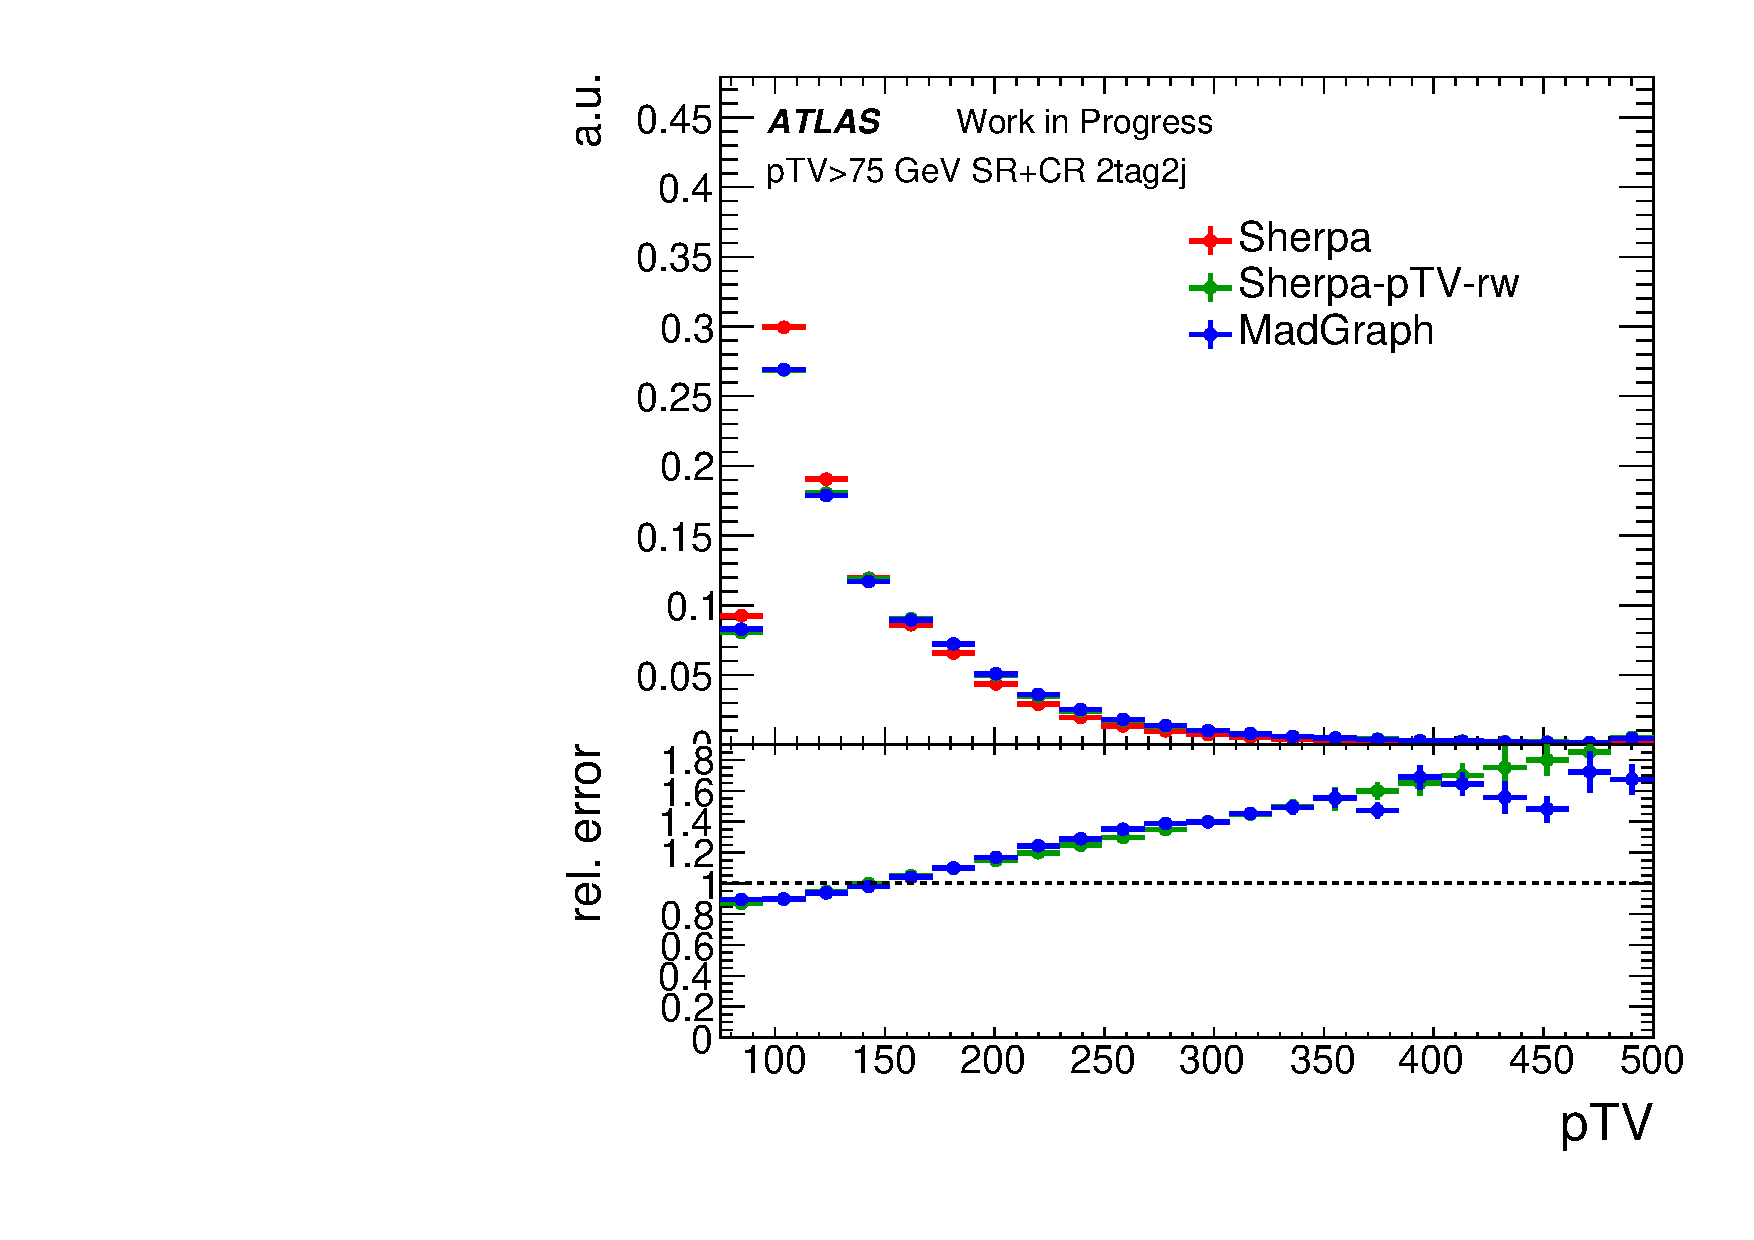
\includegraphics[width=0.45\textwidth]{1Lep_pTVreweighting_shapes/1lepton_2tag2jet_75ptv_SR+CR_pTV_bl.pdf}} 
  \subfigure[$p_T^V$ 2tag 2jet
  cc]{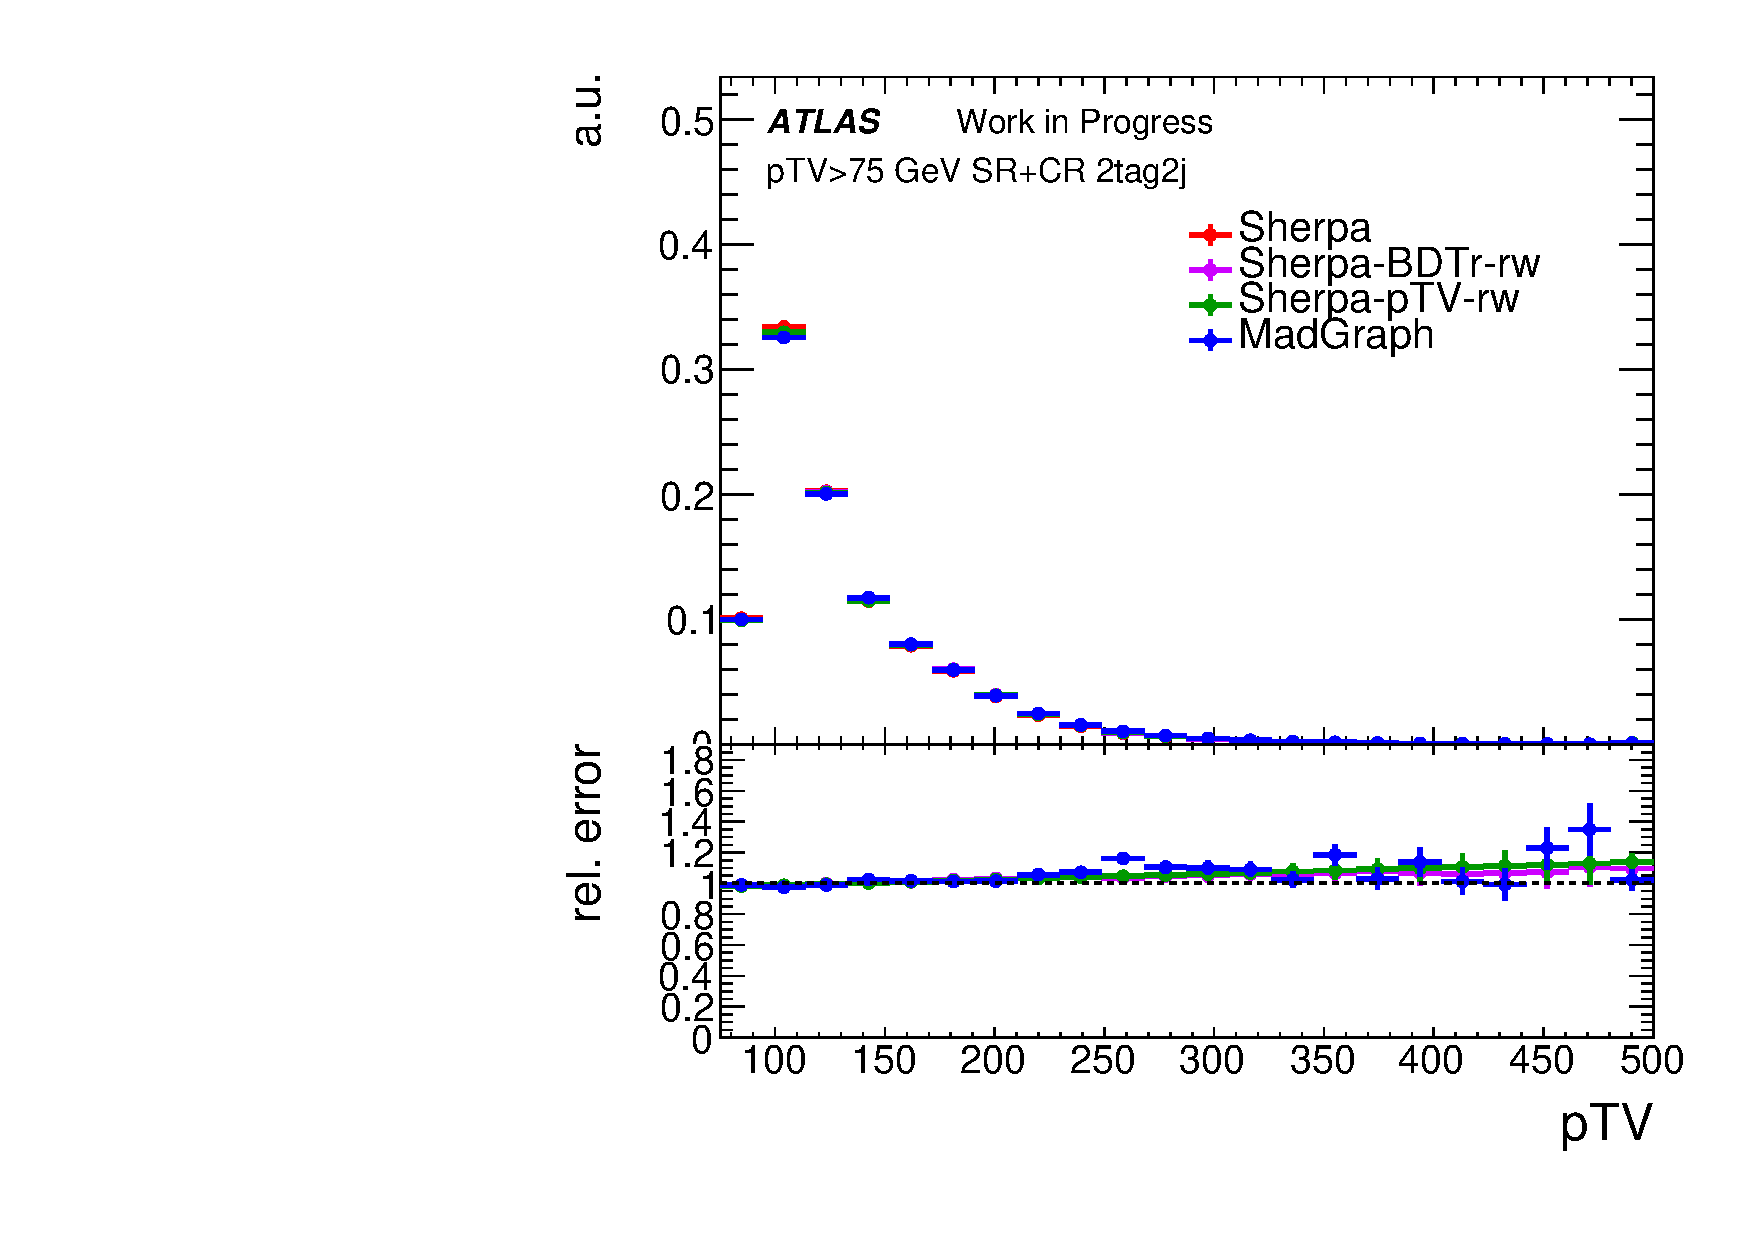
\includegraphics[width=0.45\textwidth]{1Lep_pTVreweighting_shapes/1lepton_2tag2jet_75ptv_SR+CR_pTV_cc.pdf}}
  \\
  \caption{$p_T^V$ shape systematic in the 2--jet category in the 1--lepton
    channel for each heavy flavour sub-component. The red and blue histograms
    correspond to the $p_T^V$ prediction of \textsc{Sherpa}~2.2.1 and
    \textsc{MadGraph} respectively. The $p_T^V$ shape systematic is plotted in
    green.}
  \label{fig:wjets_1lep_2jet_SysWPtVBDTr}
\end{figure}

\begin{figure}[ht!]
  \centering
  \subfigure[$p_T^V$ 2tag 3jet
  bb]{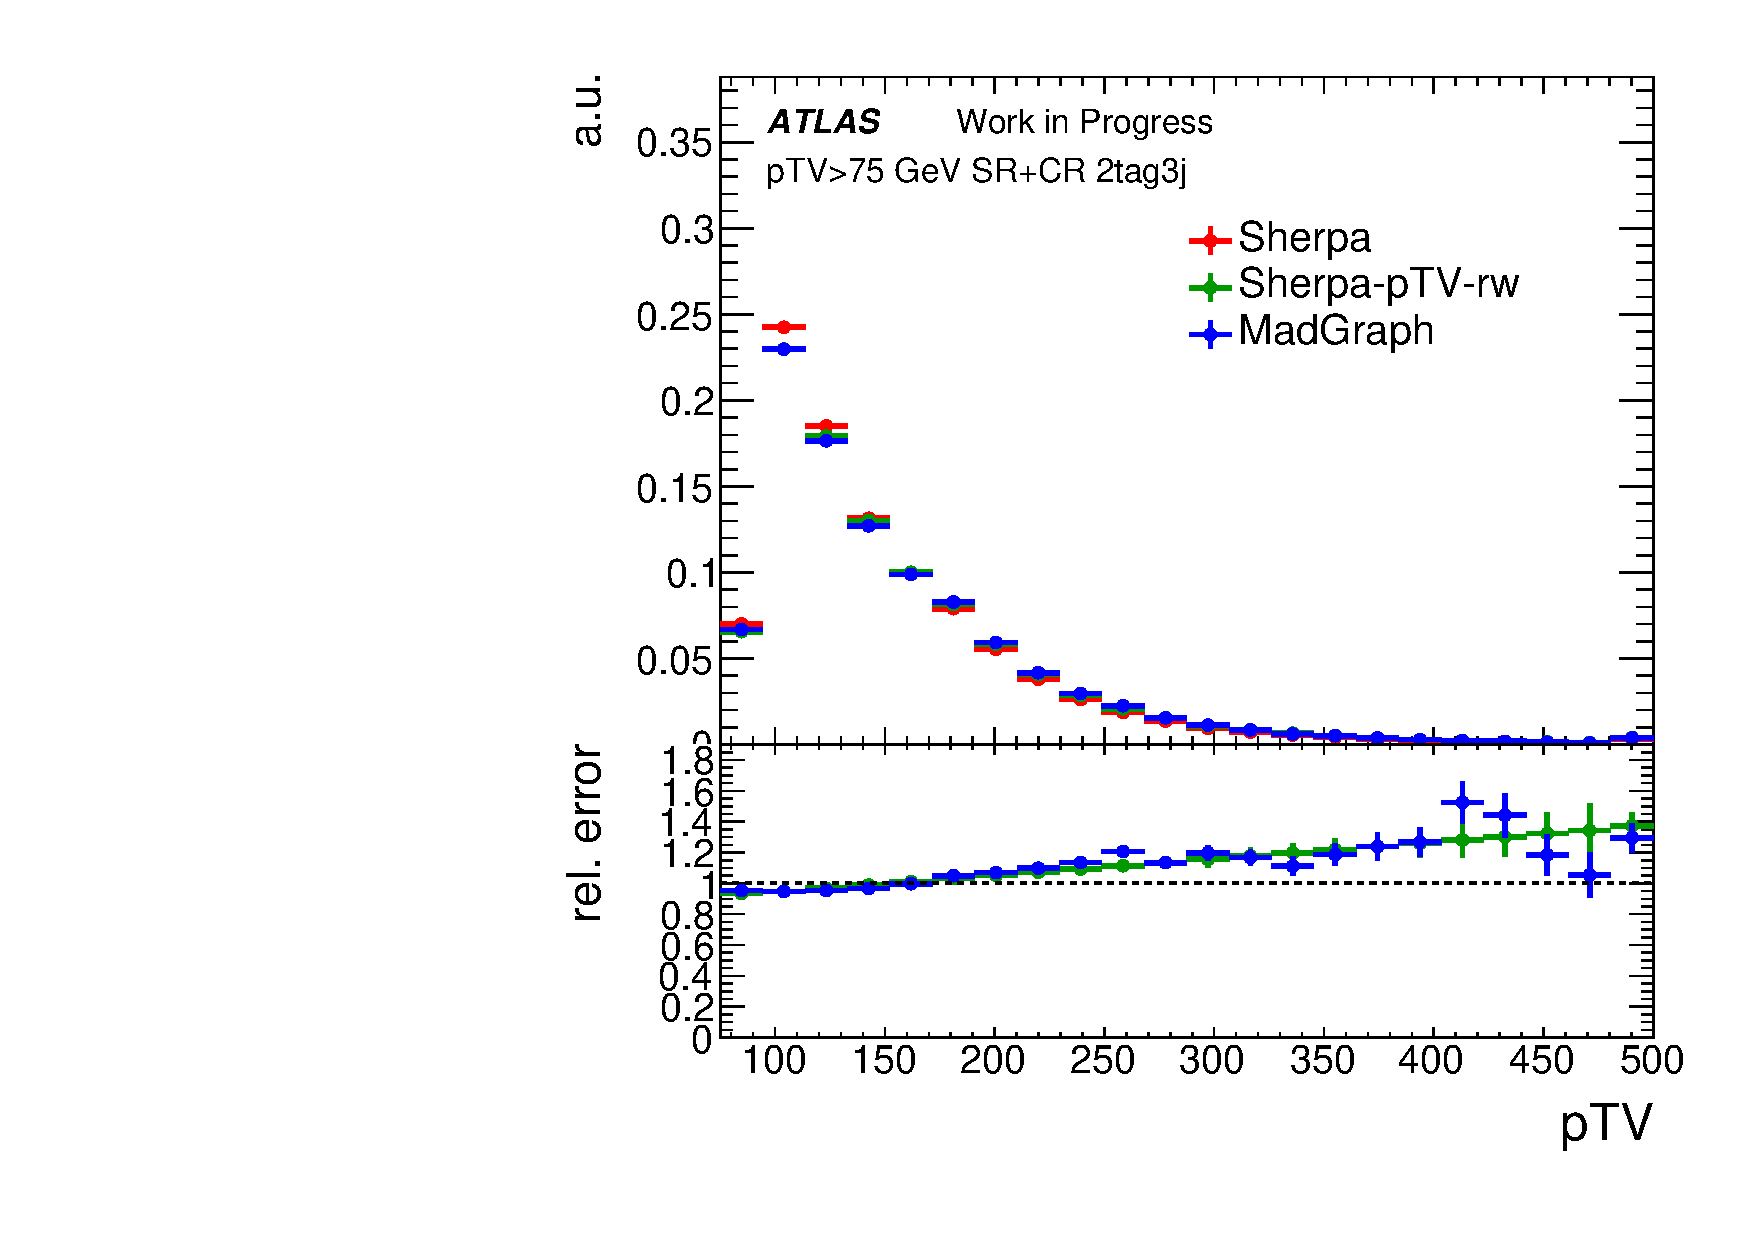
\includegraphics[width=0.45\textwidth]{1Lep_pTVreweighting_shapes/1lepton_2tag3jet_75ptv_SR+CR_pTV_bb.pdf}}
  \subfigure[$p_T^V$ 2tag 3jet
  bc]{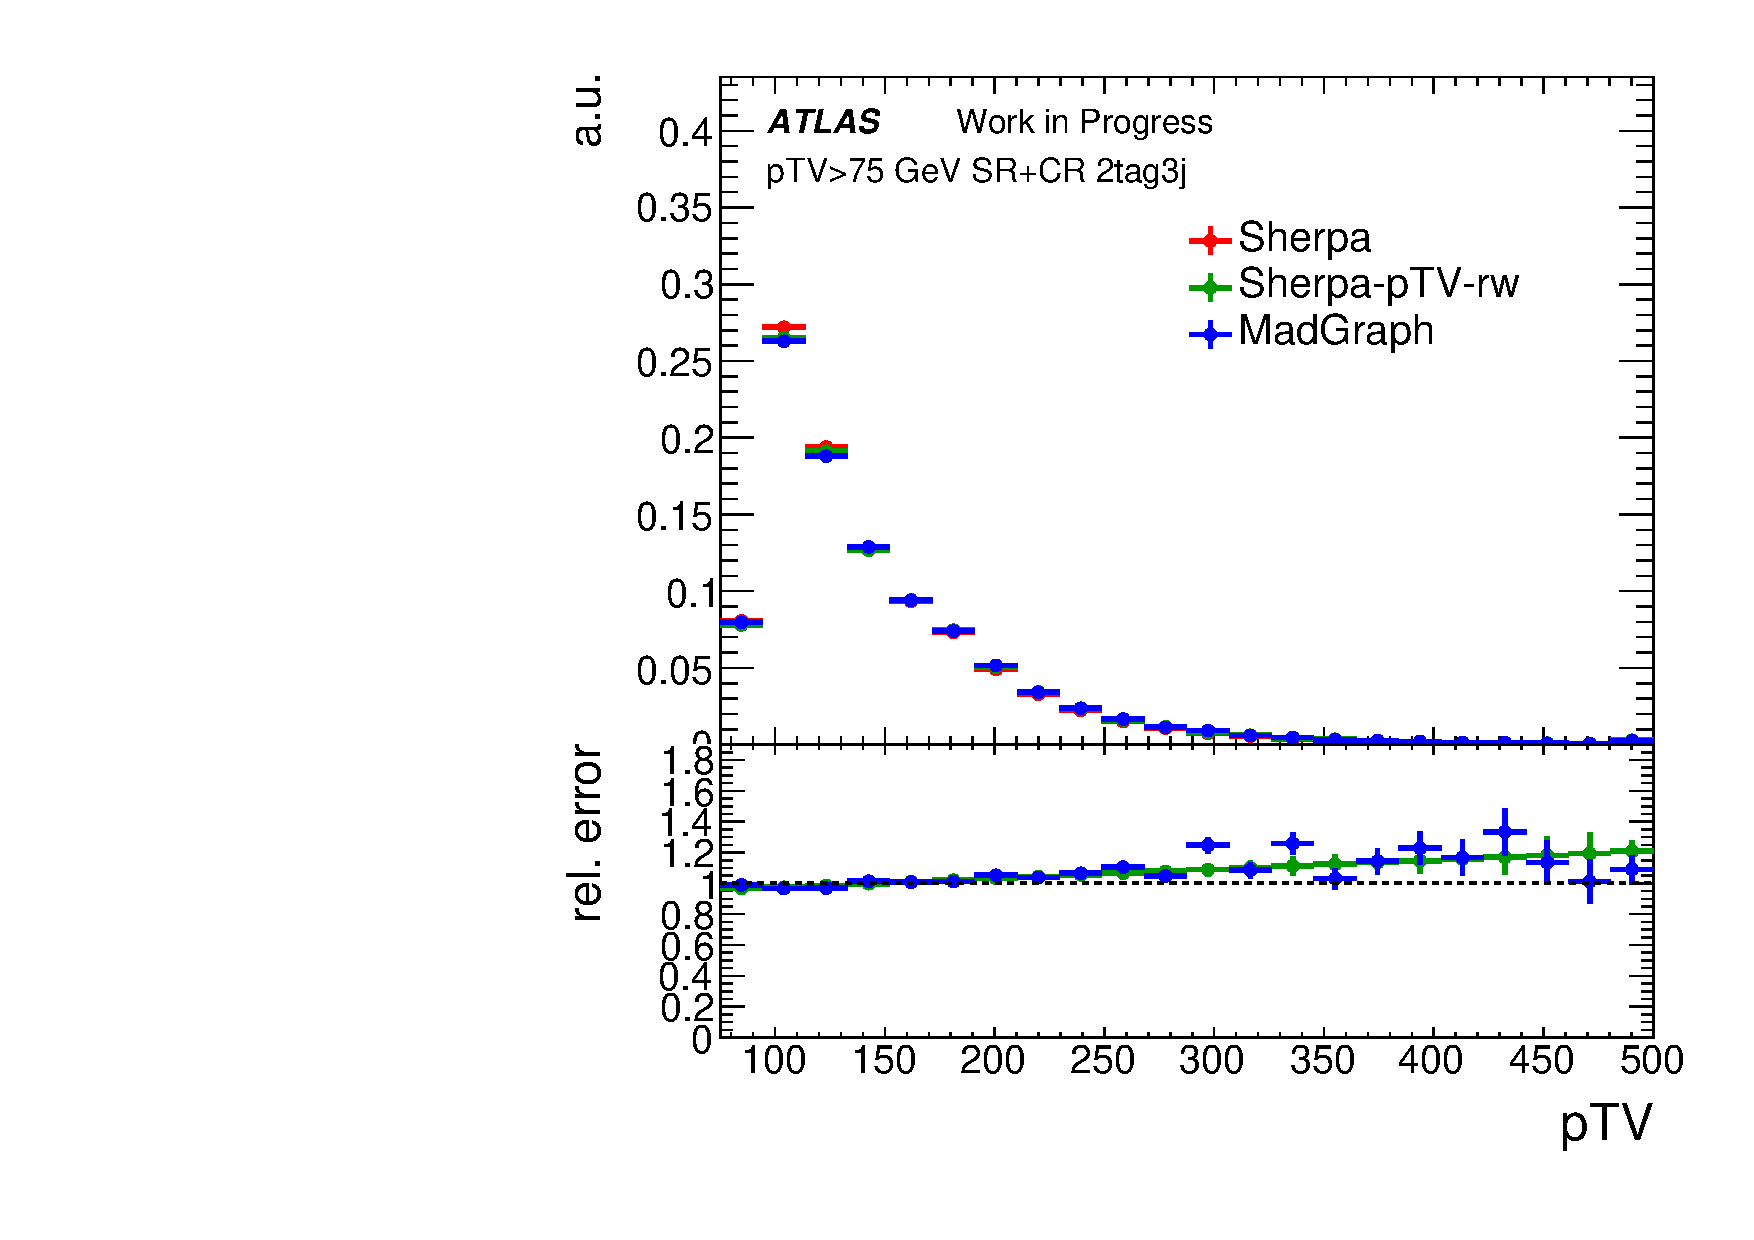
\includegraphics[width=0.45\textwidth]{1Lep_pTVreweighting_shapes/1lepton_2tag3jet_75ptv_SR+CR_pTV_bc.pdf}}
  \\
  \subfigure[$p_T^V$ 2tag 3jet
  bl]{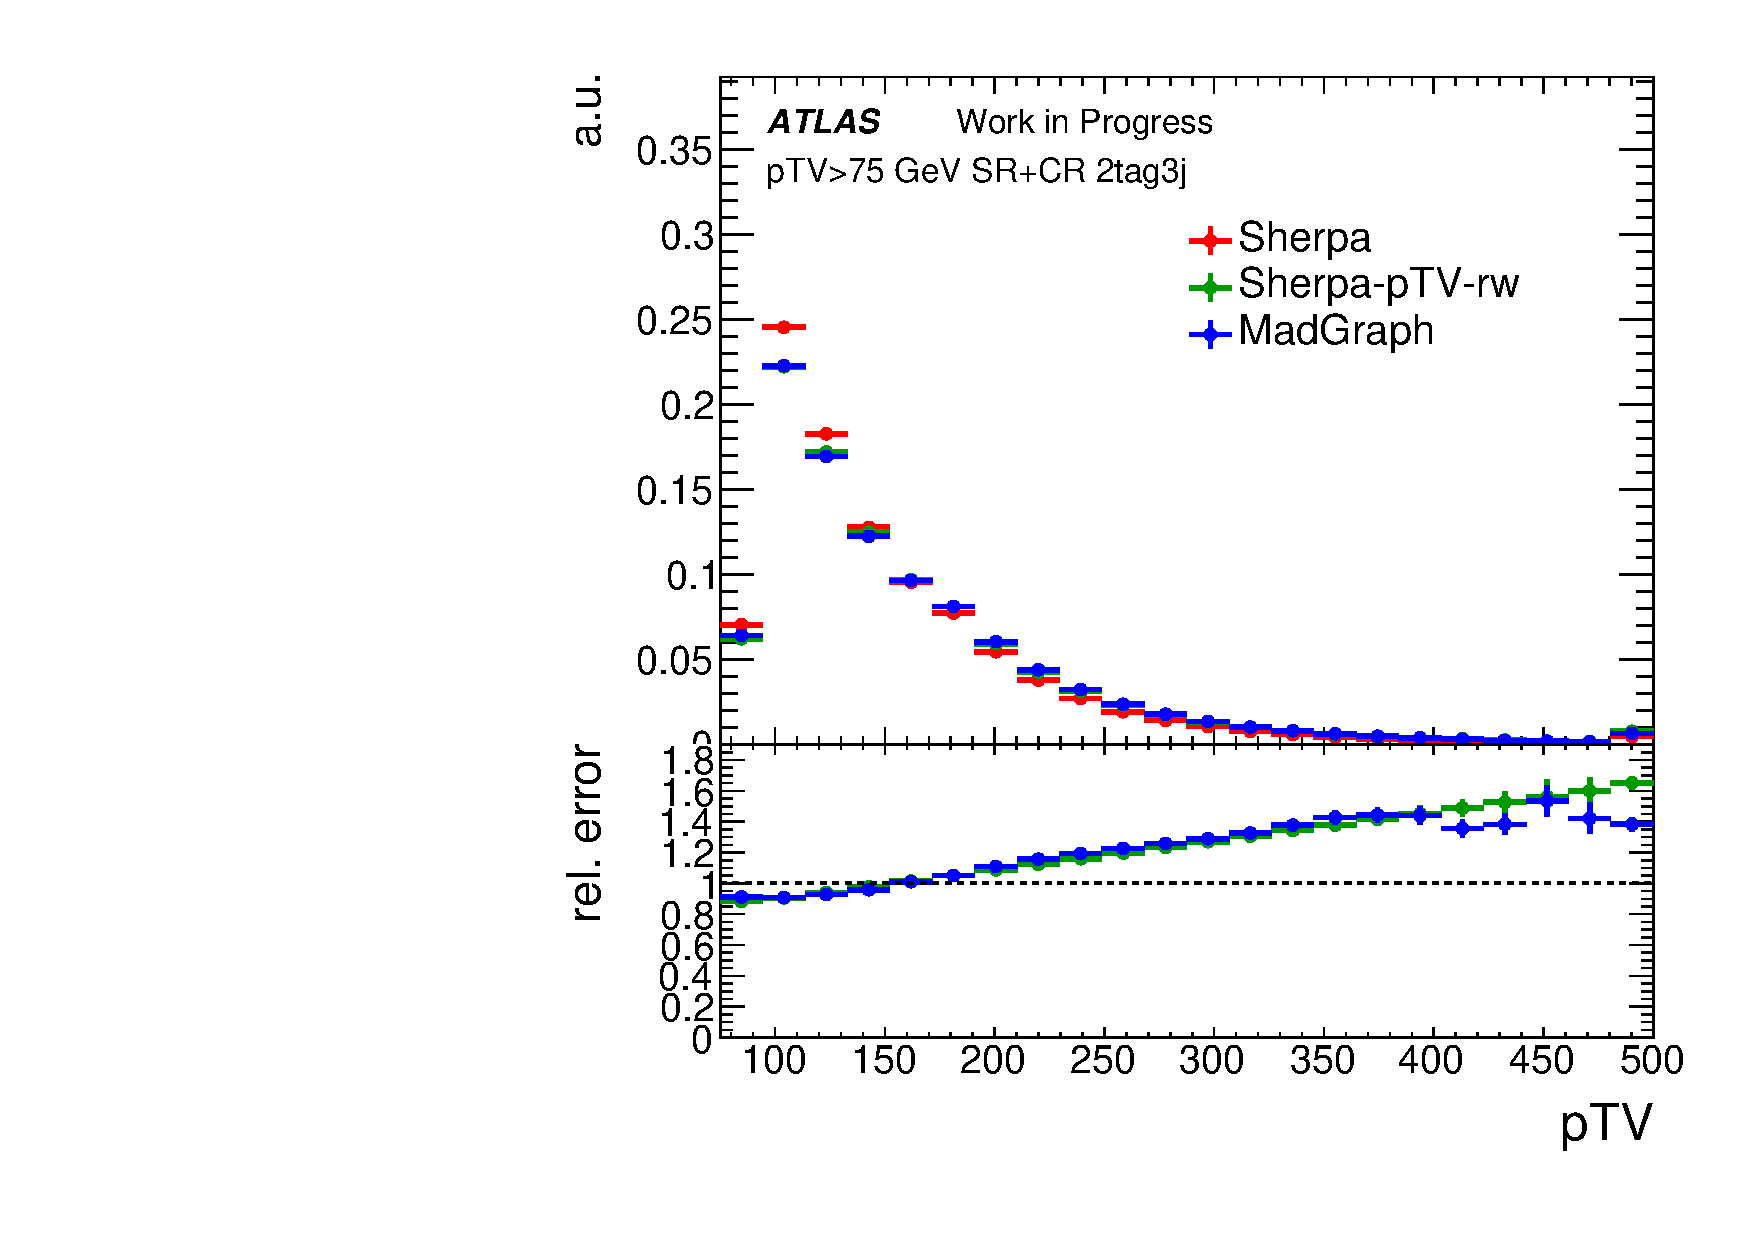
\includegraphics[width=0.45\textwidth]{1Lep_pTVreweighting_shapes/1lepton_2tag3jet_75ptv_SR+CR_pTV_bl.pdf}}
  \subfigure[$p_T^V$ 2tag 3jet
  cc]{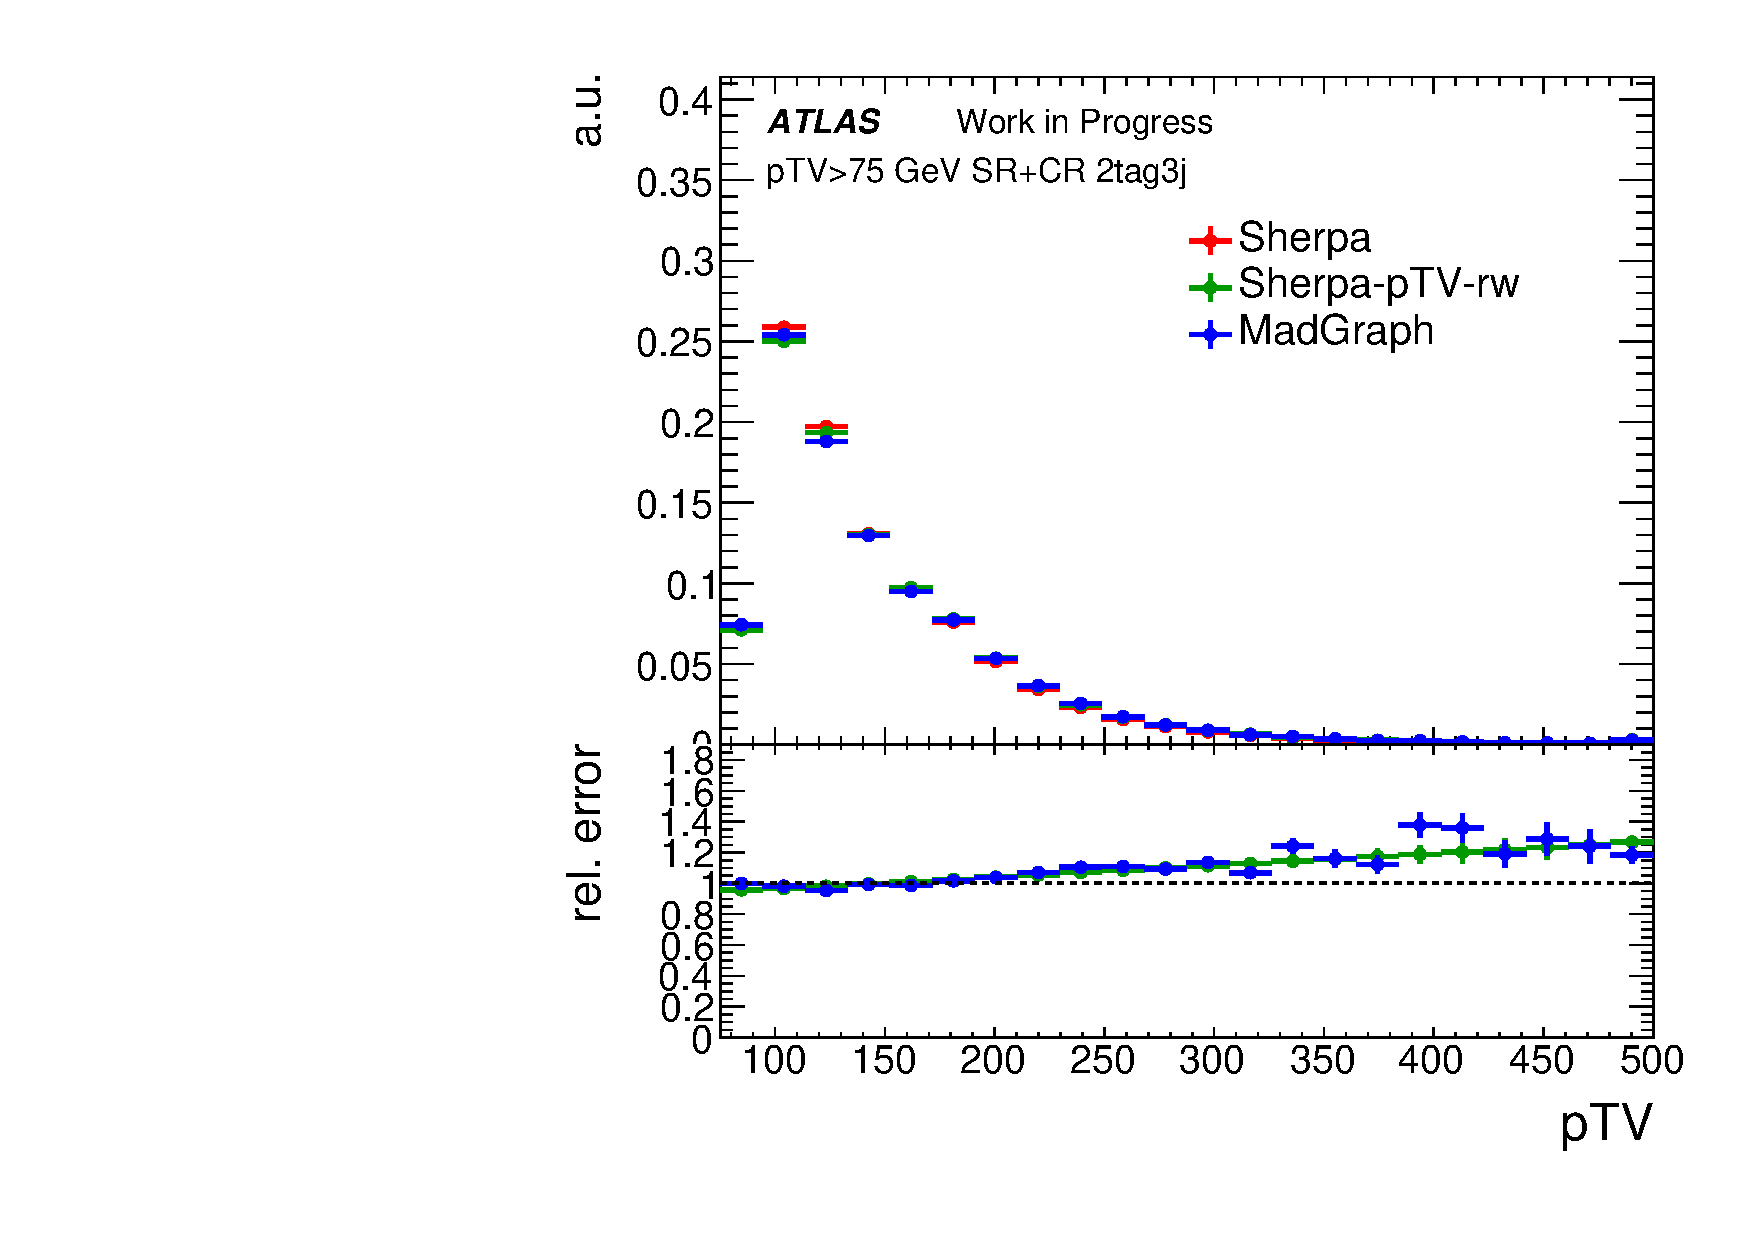
\includegraphics[width=0.45\textwidth]{1Lep_pTVreweighting_shapes/1lepton_2tag3jet_75ptv_SR+CR_pTV_cc.pdf}}
  \\
  \caption{$p_T^V$ shape systematic in the 3--jet category in the 1--lepton
    channel for each heavy flavour sub-component. The red and blue histograms
    correspond to the $p_T^V$ prediction of \textsc{Sherpa}~2.2.1 and
    \textsc{MadGraph} respectively. The $p_T^V$ shape systematic is plotted in
    green.}
  \label{fig:wjets_1lep_3jet_SysWPtVBDTr}
\end{figure}